% !TEX TS-program = pdflatex
% !TEX encoding = UTF-8 Unicode

% This is a simple template for a LaTeX document using the "article" class.
% See "book", "report", "letter" for other types of document.

\documentclass[11pt]{article} % use larger type; default would be 10pt

\usepackage[utf8]{inputenc} % set input encoding (not needed with XeLaTeX)

%%% Examples of Article customizations
% These packages are optional, depending whether you want the features they provide.
% See the LaTeX Companion or other references for full information.

%%% PAGE DIMENSIONS
\usepackage{geometry} % to change the page dimensions
\geometry{letterpaper} % or letterpaper (US) or a5paper or....
% \geometry{margin=2in} % for example, change the margins to 2 inches all round
% \geometry{landscape} % set up the page for landscape
%   read geometry.pdf for detailed page layout information

\usepackage{graphicx} % support the \includegraphics command and options

% \usepackage[parfill]{parskip} % Activate to begin paragraphs with an empty line rather than an indent

%%% PACKAGES
\usepackage{booktabs} % for much better looking tables
\usepackage{array} % for better arrays (eg matrices) in maths
\usepackage{paralist} % very flexible & customisable lists (eg. enumerate/itemize, etc.)
\usepackage{verbatim} % adds environment for commenting out blocks of text & for better verbatim
\usepackage{subfig} % make it possible to include more than one captioned figure/table in a single float
% These packages are all incorporated in the memoir class to one degree or another...

%%% HEADERS & FOOTERS
\usepackage{fancyhdr} % This should be set AFTER setting up the page geometry
\pagestyle{fancy} % options: empty , plain , fancy
\renewcommand{\headrulewidth}{0pt} % customise the layout...
\lhead{}\chead{}\rhead{}
\lfoot{}\cfoot{\thepage}\rfoot{}

%%% SECTION TITLE APPEARANCE
\usepackage{sectsty}
\allsectionsfont{\sffamily\mdseries\upshape} % (See the fntguide.pdf for font help)
% (This matches ConTeXt defaults)

%%% ToC (table of contents) APPEARANCE
\usepackage[nottoc,notlof,notlot]{tocbibind} % Put the bibliography in the ToC
\usepackage[titles,subfigure]{tocloft} % Alter the style of the Table of Contents
\renewcommand{\cftsecfont}{\rmfamily\mdseries\upshape}
\renewcommand{\cftsecpagefont}{\rmfamily\mdseries\upshape} % No bold!

%%% END Article customizations

\renewcommand\thesubsection{\alph{subsection})}

%%% The "real" document content comes below...
\usepackage[normalem]{ulem}

\title{Assignment 4: Linear Least Squares Problems}
\author{ Gregory \uline{Smetana} \\ID 1917370 \\ ACM 106a }
%\date{} % Activate to display a given date or no date (if empty),
         % otherwise the current date is printed 

\usepackage{fancyhdr}
\usepackage{lastpage}

\usepackage{../mcode}

\usepackage{mathtools}
\pagestyle{fancy}
\lhead{Gregory \uline{Smetana}}
\rhead{ID 1917370 }


\begin{document}


\maketitle


\section{The Pseudoinverse}
Suppose that $A \in \mathbf{R}^{m\times n}$ with $m > n$ and full column rank (rank($A$) = $n$). %The pseudoinverse is defined as $A^{\dagger} = (A^{T}A)^{-1}A^T$

\subsection{} %1a
The Frobenius norm is defined as
\begin{equation}
\| M \|_F^2 = \sum_i \sum_j M_{ij}^2
\end{equation}
If the columns of $M = \left [ m_1, m_2, ... , m_m \right ]$, the Frobenius norm of M may be expressed as the sum of the vector 2-norms of the columns of M
\begin{equation}
\|M \|_F^2 = \sum_j \|m_j \|_2^2
\end{equation}
The Frobenius norm of the matrix product $AX-I$ is
\begin{equation}
\|AX-I\|_F^2 = \sum_j^m \| (AX-I)_j \|_2^2
\end{equation}
If the columns of $X = \left [x_1, x_2, ... , x_m \right ]$, and $e_j$ are the standard basis vectors, this may be written
\begin{equation}
\|AX-I\|_F^2 = \sum_j^m \| (Ax_j-e_j) \|_2^2
\end{equation}
All norms have the property $\| X \| \ge 0$, so the $X$ that minimizes $\|AX-I\|_F^2$ will have columns $x_j$ that minimize each term in the sum. As discussed in class, the $x$ that minimizes $\| Ax -b \|_2^2$ for rank deficient $A$ is 
\begin{equation}
x = A^\dagger b
\end{equation}
where the Moore-Penrose generalized inverse inverse is $A^\dagger = (A^{T}A)^{-1}A^T$. Therefore, the columns of $X$ are the columns of $A^\dagger$, and we have shown that $X=A^\dagger$ minimizes
\begin{equation}
\substack{\min \\X \in \mathbf{R}^{n \times m}} \| AX -I \|_{F}
\end{equation}

\subsection{} %1b
The SVD of $A$ states
\begin{equation}
A = U \Sigma V^T
\end{equation}
where
\begin{itemize}
\item $U \in \mathbf{R}^{m\times n}$ such that $U^T U = I$
\item $V \in \mathbf{R}^{n\times n}$ such that $V^T V = I$
\item $\Sigma =$ Diag$(\sigma_1, \sigma_2, ... , \sigma_n)$ where $\sigma_1 \ge \sigma_2 \ge ... \ge \sigma_n \ge 0$. 
\end{itemize}
The corresponding pseudoinverse of $A$ is
\begin{equation}
A^\dagger = V \Sigma^{-1} U^T
\end{equation}
Expanding the product $(A A^\dagger )A $,
\begin{equation}
\begin{split}
(A A^\dagger )A &= (U \Sigma V^T )(V \Sigma^{-1} U^T)( U \Sigma V^T) \\
& = U \Sigma \Sigma^{-1} \Sigma V^T \\
& = U \Sigma V^T \\
& = A
\end{split}
\end{equation}
\begin{equation}
\boxed{(A A^\dagger ) A = A}
\end{equation}

\subsection{} %1c
Expanding the product $A^T(A A^\dagger )$,
\begin{equation}
\begin{split}
A^T(A A^\dagger ) &= (U \Sigma V^T )^T (U \Sigma V^T ) (V \Sigma^{-1} U^T) \\
&= (V \Sigma^T U^T ) (U \Sigma V^T ) (V \Sigma^{-1} U^T) \\
&= V \Sigma^T \Sigma  \Sigma^{-1} U^T \\
&= V \Sigma^T  U^T \\
&= (U \Sigma  V^T)^T \\
&= A^T 
\end{split}
\end{equation}
\begin{equation}
\boxed{A^T(A A^\dagger ) = A^T}
\end{equation}

\section{The underdetermined problem}
Suppose that $A \in \mathbf{R}^{m \times n}$ with $m < n$. If $A$ is full row rank (rank($A$) = m), the matrix $A^T  \in \mathbf{R}^{n\times m}$ has full column rank. Using the SVD of $A^T$,
\begin{equation}
A^T = U \Sigma V^T
\end{equation}
where
\begin{itemize}
\item $U \in \mathbf{R}^{n\times m}$ such that $U^T U = I$
\item $V \in \mathbf{R}^{m\times m}$ such that $V^T V = I$%, and the columns of $V$ corresponding to zero singular values form an orthonormal basis for the null space of $A^T$
\item $\Sigma =$ Diag$(\sigma_1, \sigma_2, ... , \sigma_m)$ where $\sigma_1 \ge \sigma_2 \ge ... \ge \sigma_m \ge 0$. 
\end{itemize}
The matrix $A$ may be expressed
\begin{equation}
A = V \Sigma U^T
\end{equation}
Any solution $x$ to the linear system $Ax=b$ may be written in the form $x=x_1+x_2$, where $x_1 \in $ Col($A^T$) and $x_2 \in $ Null($A$)
\begin{equation}
\| Ax-b\|_2^2 = \| V \Sigma U^T (x_1 +x_2) -b \|_2^2
\end{equation}
 The columns of $U$ are a set of basis vectors for the range of $A^T$, so the vector $x_2$ is orthogonal to the columns of $U$
\begin{equation}
\| Ax-b\|_2^2 = \| V \Sigma U^T x_1 - b \|_2^2
\end{equation}
Choosing the minimum norm solution from this subspace,
\begin{equation}
\begin{split}
x &= U \Sigma^{-1} V^T b \\
& = U \Sigma \Sigma^{-1} \Sigma^{-1} V^T b \\
& = U \Sigma V^T V^{-T} \Sigma^{-1}  U U^T \Sigma^{-1} V^T b \\
& = U \Sigma V^T( V \Sigma  U^T U \Sigma V^T )^{-1} b \\
& = A^T(A A^T)^{-1} b
\end{split}
\end{equation}
So we have shown the minimum 2-norm solution of $Ax=b$ is equal to
\begin{equation}
\boxed{x = A^\dagger b}
\end{equation}
where $A^\dagger = A^T (A A^T)^{-1}$


\section{Polynomial approximation}
Polynomials of order $m$ may be fit to functions sampled with values $b_i$ at points $t_i$  by solving the least squares problem
\begin{equation}
x = \arg \substack{\min \\x \in \mathbf{R}^{m}} \| Ax -b\|_{2}
\end{equation}
where $A \in \mathbf{R}^{n \times m}$ is the matrix with $(i,j)th$ entry equal to $A_{i,j}=t_i^{j-1}$
\subsection{} %3a
The normal equations $A^T A x = A^T b$ were solved using a Cholesky factorization in the first part of this problem.
\subsection{} %3b
A Householder-based QR factorization of $A$ was used to solve the least squares problem in the second part. A version of the algorithm was used that avoids any explicit computation of the projection matrices. In both algorithms, triangular systems were solved using the Matlab backslash command. The code is attached as an Appendix.

The function $f(t) = \sin(4t)$ and was sampled at $n=51$ points on the interval [0,1]. The function and approximating polynomials of each method for values $m=3,7,12$ are plotted in Figures 1-3. The results for the solution coefficient vector $x$, the norm of the residual, and time required to obtain the approximation for each method  for values $m=3,7,12$ are summarized in Tables 1-3.

\begin{figure}[h!]
  \centering
    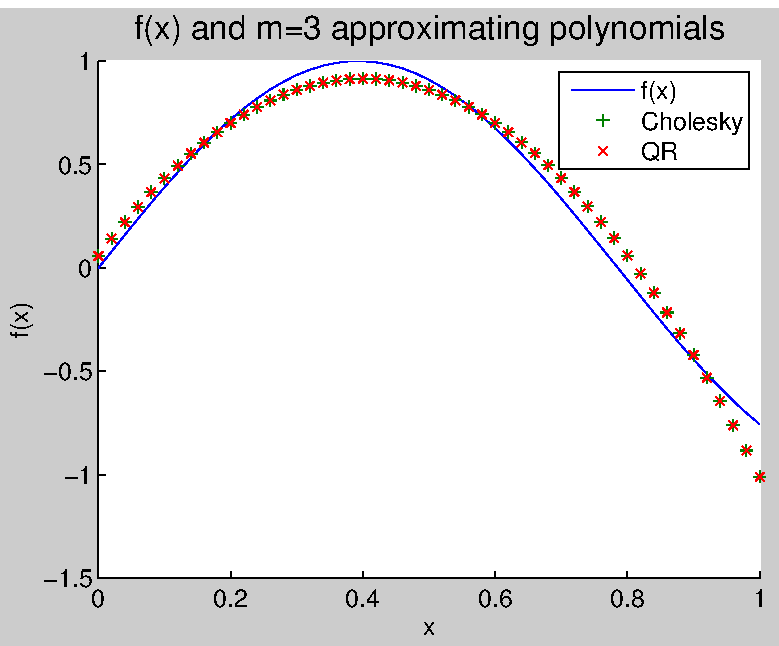
\includegraphics[width=0.7\textwidth]{p3_m=3}
  \caption{}
\end{figure}

\begin{figure}[h!]
  \centering
    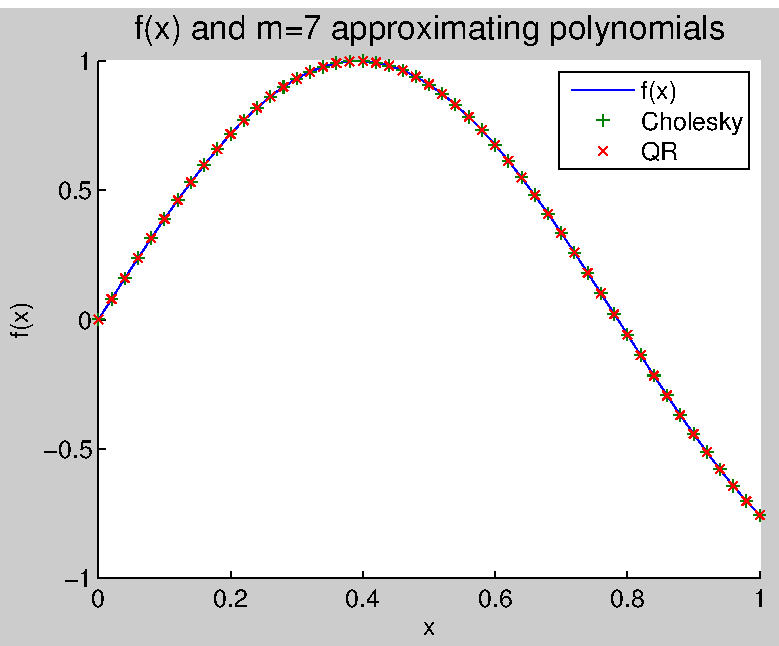
\includegraphics[width=0.7\textwidth]{p3_m=7}
  \caption{}
\end{figure}

\begin{figure}[h!]
  \centering
    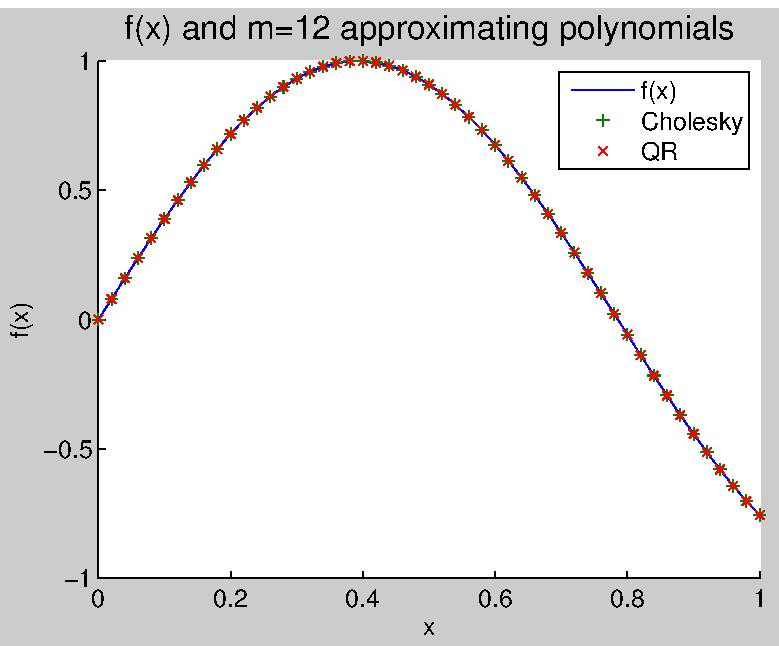
\includegraphics[width=0.7\textwidth]{p3_m=12}
  \caption{}
\end{figure}

\begin{table}[h!]
\centering
\begin{tabular}{| c | l | l | }\hline
 & Cholesky factorization & QR factorization \\ \hline
solution vector $x$ &5.773287988489395e-02 &     5.773287988488140e-02
 \\ 
& 4.281921761790140e+00 &      4.281921761790207e+00
\\
&-5.349578523794193e+00  &     -5.349578523794256e+00
\\ \hline
 $\|Ax - b \|_2$ &5.811882658961149e-01 &      5.811882658961154e-01
\\ \hline
Time required [$\mu$s] & 810 &1516 \\ \hline
Condition number & $\kappa_2(A^T A )$ = 4.867618438401785e+02& $\kappa_2(A )$ =     2.206267988799603e+01
 \\ \hline
\end{tabular}
\caption{Comparison of Cholesky and QR methods for $m=3$}
\end{table}

\begin{table}[h!]
\centering
\begin{tabular}{| c | l | l | }\hline
 & Cholesky factorization & QR factorization \\ \hline
solution vector $x$ &   1.656380936174698e-04  &         1.656380962030799e-04\\
&    3.989420649671397e+00  &      3.989420649508054e+00     \\
&     1.229658456163471e-01  &      1.229658474860089e-01     \\
&    -1.112693941751450e+01  &      -1.112693942551486e+01    \\
&     2.760391884291479e-01  &        2.760392040232638e-01   \\
&     1.048354404629816e+01  &      1.048354403224540e+01  \\ 
&    -4.502277252395971e+00 &     -4.502277247641723e+00\\ \hline
 $\|Ax - b \|_2$ &     7.468336144166766e-04 &       7.468336144165733e-04
  \\ \hline
Time required [$\mu$s] &  127 & 580 \\ \hline
Condition number & $\kappa_2(A^T A )$ =     3.915604824294044e+08 & $\kappa_2(A )$ =       1.978788728823597e+04
 \\ \hline
\end{tabular}
\caption{Comparison of Cholesky and QR methods for $m=7$}
\end{table}

\begin{table}[h!]
\centering
\begin{tabular}{| c | l | l | }\hline
 & Cholesky factorization & QR factorization \\ \hline
solution vector $x$ & -6.671131127896551e-09&       -2.665211567614457e-09     \\
 &    4.000002325585443e+00&         4.000001205956912e+00    \\
 &   -9.800632713093781e-05&       -5.645186915616958e-05    \\
 &   -1.066503428065786e+01&        -1.066564308017487e+01    \\
 &   -1.430283744924931e-02&       -9.655654437952179e-03     \\
&     8.608393589186797e+00&        8.587449519298678e+00     \\
&    -2.525855838422283e-01&          -1.932254237565274e-01  \\
&      -2.686800494913550e+00&      -2.795535730790732e+00    \\
&      -8.430701648396042e-01 &       -7.145141657078831e-01   \\
&       1.550721728828908e+00 &      1.456008851886011e+00     \\
&      -5.014643416298591e-01&     -4.619239047002904e-01  \\ 
&      4.743557764659213e-02 &      4.029233913304647e-02 \\ \hline
 $\|Ax - b \|_2$ &      2.448105425893064e-08&        1.743034423482307e-08 \\ \hline
Time required [$\mu$s] &  288& 2596 \\ \hline
Condition number & $\kappa_2(A^T A )$ =     1.280614687904160e+16 & $\kappa_2(A )$ =       1.171893555129648e+08
 \\ \hline
\end{tabular}
\caption{Comparison of Cholesky and QR methods for $m=12$}
\end{table}

\clearpage
Visually, the quality of the approximation of both methods for $m>3$ appears to be very good. The values of the residual and coefficients at $m=3$ and $m=7$ are similar to at least 10 digits for both methods, but the residual for the Cholesky factorization is higher than the QR factorization at $m=12$. The product $A^TA$ squares the condition number. Therefore, the Cholesky factorization solving the normal equations is less well conditioned than the QR factorization of $A$ and is not well suited for large values of $m$.

As discussed in class, the QR decomposition requires $2n^2m - 2/3 n^3 + O(m^2)+O(n^2)$ operations. The cost of computing the product $A^TA$ and performing the Cholesky factorization is $ m^2n + 1/3 m^3+ O(m^2)$. This analysis leads us to believe that the time required by the Cholesky method should increase more rapidly with $m$ than the QR method, but the times required for the Cholesky and QR factorization for different values of $m$ do not show any clear trends. This is likely because the the cost of memory operations is relatively large, and the time will be sensitive to background programs running. An average of many trials may give better results.

\clearpage
\appendix
\section{Smetana\_Gregory\_1917370\_A4\_P3\_DIARY.txt}
\lstinputlisting{../Smetana_Gregory_1917370_A4_P3_DIARY.txt}

\section{Smetana\_Gregory\_1917370\_A4\_P3.m}
\lstinputlisting{../Smetana_Gregory_1917370_A4_P3.m}

\section{householder.m}
\lstinputlisting{../householder.m}

\section{getQb.m}
\lstinputlisting{../getQb.m}

\end{document}

